
% l = 8
% \mbox{}\\[-0.75in]
\begin{figure}[!b]
\begin{center}
\subfloat{
\resizebox{8cm}{4.5cm}{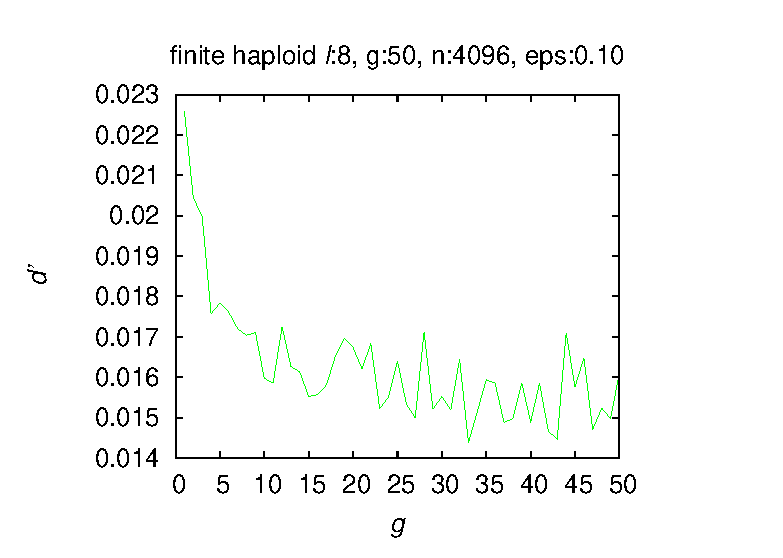
\includegraphics{figures/eps/vio/chi/b8/e0.1/n00004096_fin_hap.eps}}} \hspace{-3em}%
\subfloat{
\resizebox{8cm}{4.5cm}{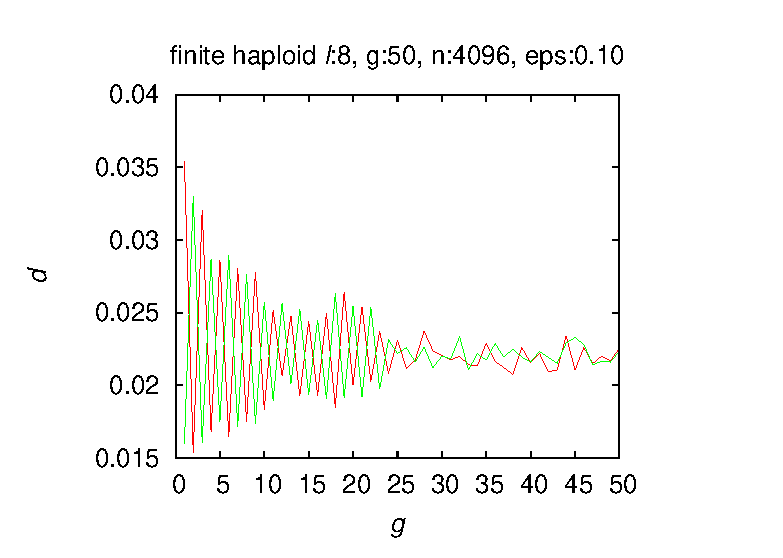
\includegraphics{figures/eps/vio/chi/b8/e0.1/n00004096_fin_hap_wovio.eps}}}\vspace{-1em} \hspace{-3em}%
\end{center}
\begin{center}
\subfloat{
\resizebox{8cm}{4.5cm}{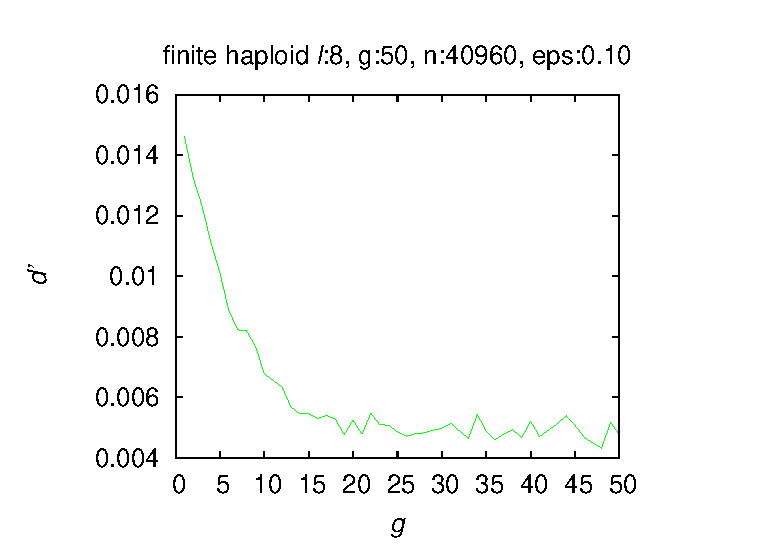
\includegraphics{figures/eps/vio/chi/b8/e0.1/n00040960_fin_hap.eps}}} \hspace{-3em}%
\subfloat{
\resizebox{8cm}{4.5cm}{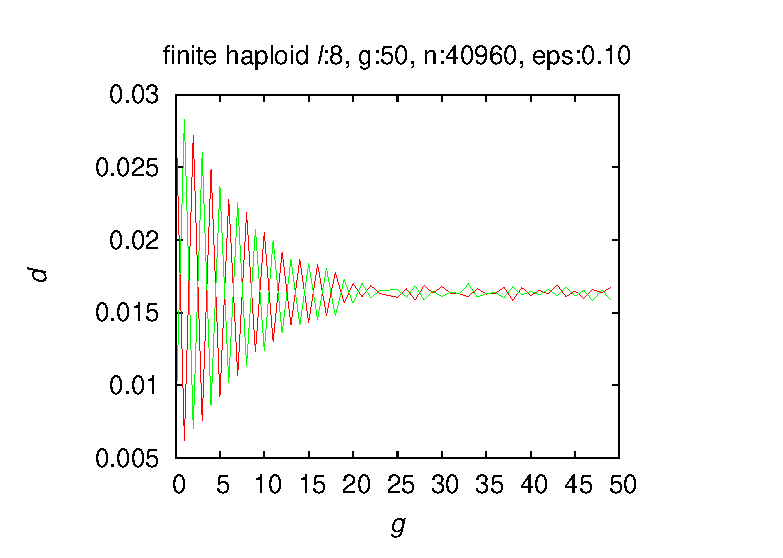
\includegraphics{figures/eps/vio/chi/b8/e0.1/n00040960_fin_hap_wovio.eps}}}\vspace{-1em} \hspace{-3em}%
\end{center}

\begin{center}
\subfloat{
\resizebox{8cm}{4.5cm}{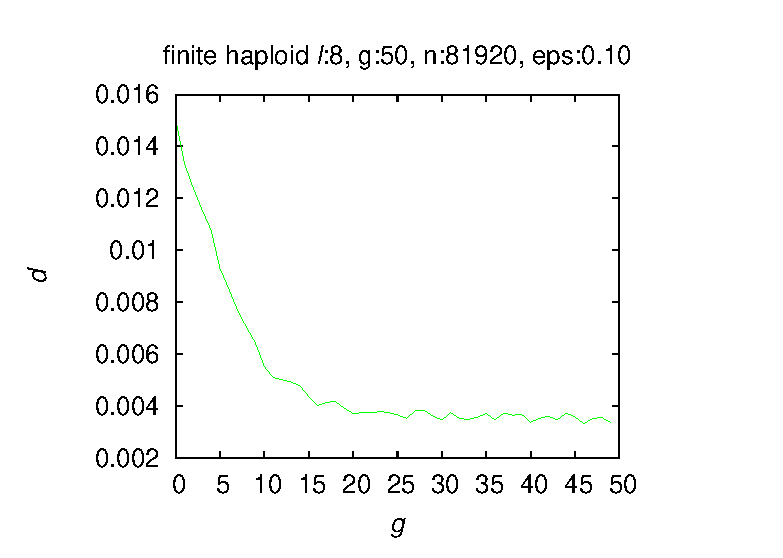
\includegraphics{figures/eps/vio/chi/b8/e0.1/n00081920_fin_hap.eps}}} \hspace{-3em}%
\subfloat{
\resizebox{8cm}{4.5cm}{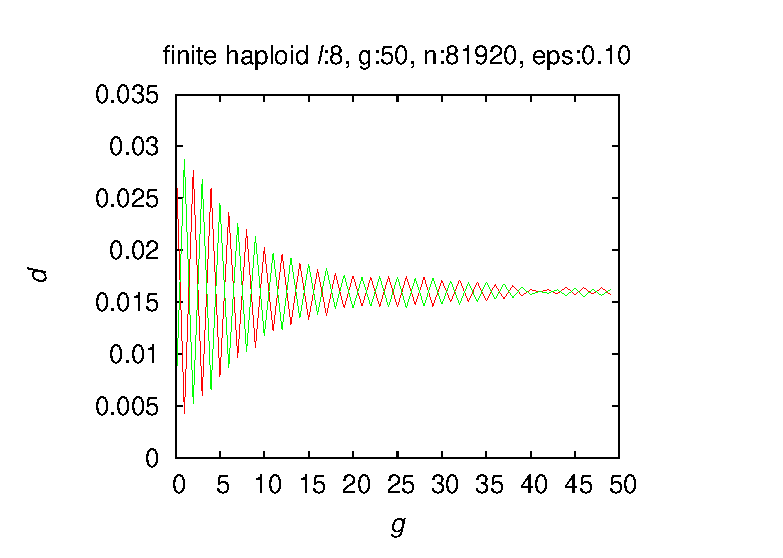
\includegraphics{figures/eps/vio/chi/b8/e0.1/n00081920_fin_hap_wovio.eps}}}\vspace{-1em} \hspace{-3em}%
\end{center}

\begin{center}
\subfloat{
\resizebox{8cm}{4.5cm}{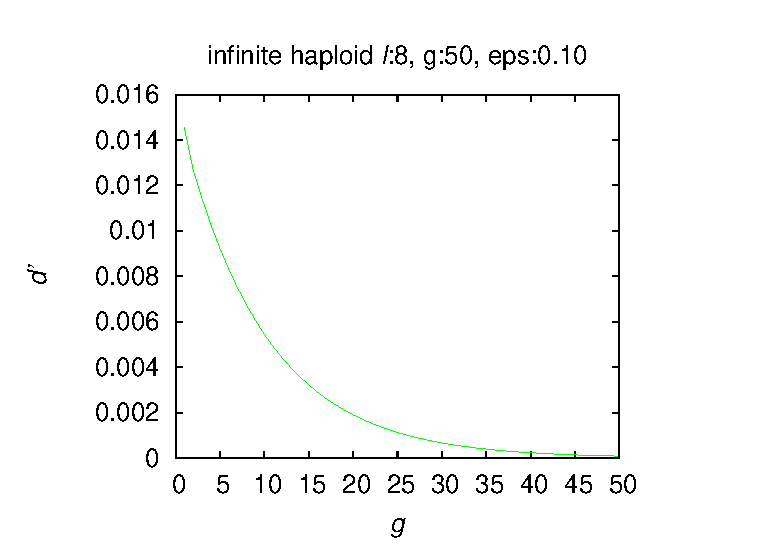
\includegraphics{figures/eps/vio/chi/b8/e0.1/inf_hap.eps}}}\hspace{-3em}%
\subfloat{
\resizebox{8cm}{4.5cm}{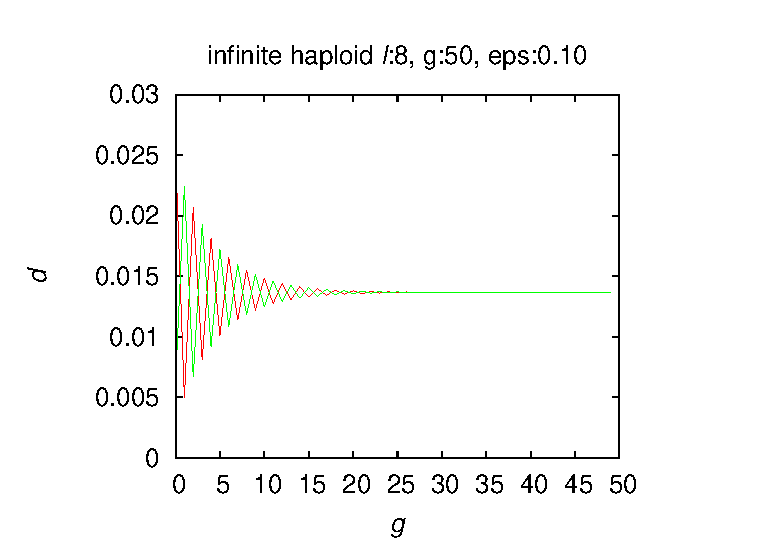
\includegraphics{figures/eps/vio/chi/b8/e0.1/inf_hap_wovio.eps}}}\vspace{-0.5em} \hspace{-3em}%


\caption[\textbf{Infinite and finite haploid population behavior for $\bm{\chi}$ violation, $\ell = 8$ and $\bm{\epsilon} = 0.1$}]
{\textbf{Infinite and finite haploid population behavior for $\bm{\chi}$ violation, $\ell = 8$ and $\bm{\epsilon} = 0.1$:} 
  In left column, $d'$ is distance of finite or infinite population to limit $\bm{z}^\ast$ for $g$ generations. 
  In right column, $d$ is distance of finite or infinite population to limits $\bm{p}^\ast$ and $\bm{q}^\ast$. Green line is distance to $\bm{p*}$ and red line is distance to $\bm{q*}$.}
\label{oscillation_8h_vio_chi_0.1}
\end{center}
\end{figure}

% l = 10

\begin{figure}[h]
\begin{center}
\subfloat{
\resizebox{8cm}{4.5cm}{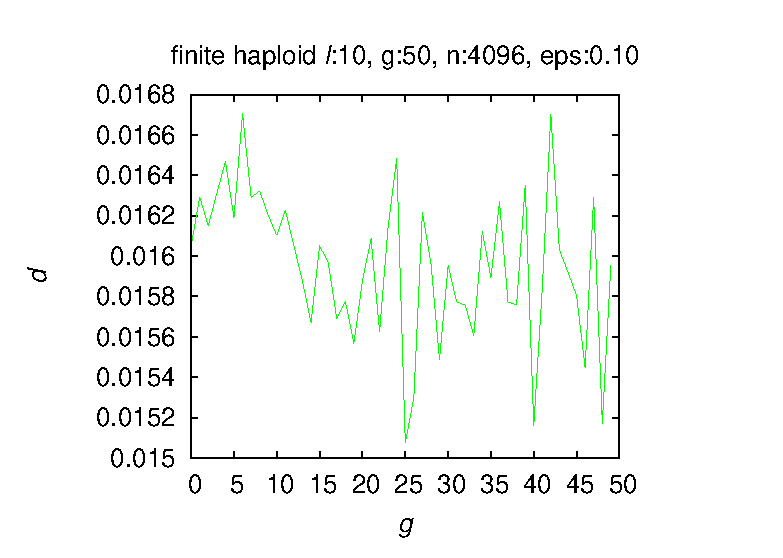
\includegraphics{figures/eps/vio/chi/b10/e0.1/n00004096_fin_hap.eps}}} \hspace{-3em}%
\subfloat{
\resizebox{8cm}{4.5cm}{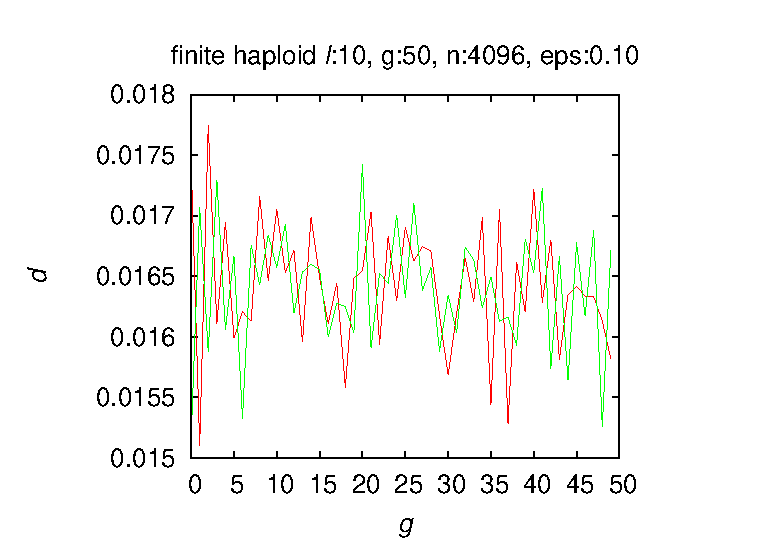
\includegraphics{figures/eps/vio/chi/b10/e0.1/n00004096_fin_hap_wovio.eps}}}\vspace{-1em} \hspace{-3em}%
\end{center}
\begin{center}
\subfloat{
\resizebox{8cm}{4.5cm}{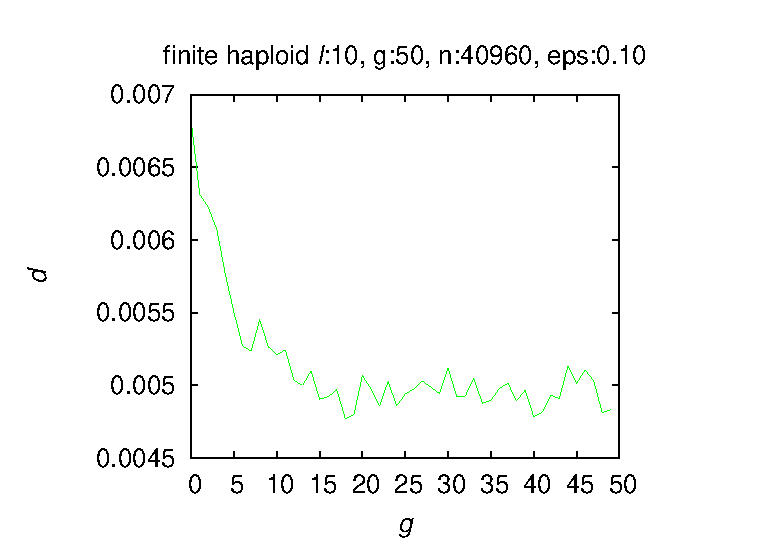
\includegraphics{figures/eps/vio/chi/b10/e0.1/n00040960_fin_hap.eps}}} \hspace{-3em}%
\subfloat{
\resizebox{8cm}{4.5cm}{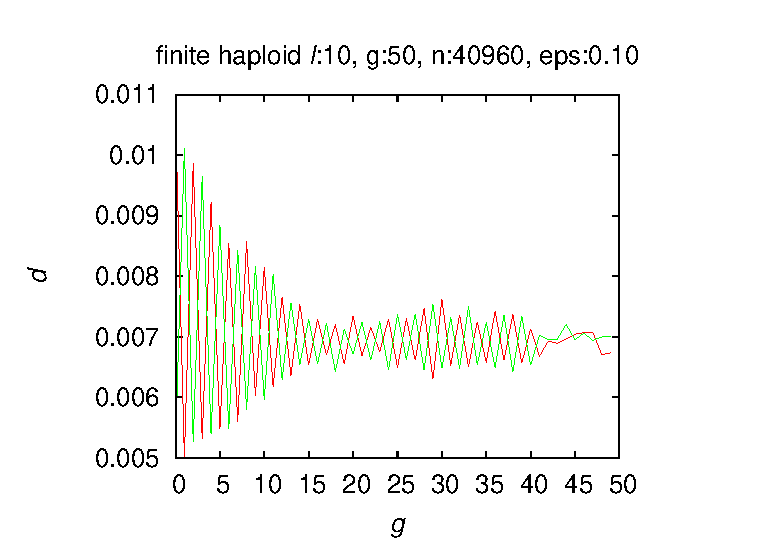
\includegraphics{figures/eps/vio/chi/b10/e0.1/n00040960_fin_hap_wovio.eps}}}\vspace{-1em} \hspace{-3em}%
\end{center}

\begin{center}
\subfloat{
\resizebox{8cm}{4.5cm}{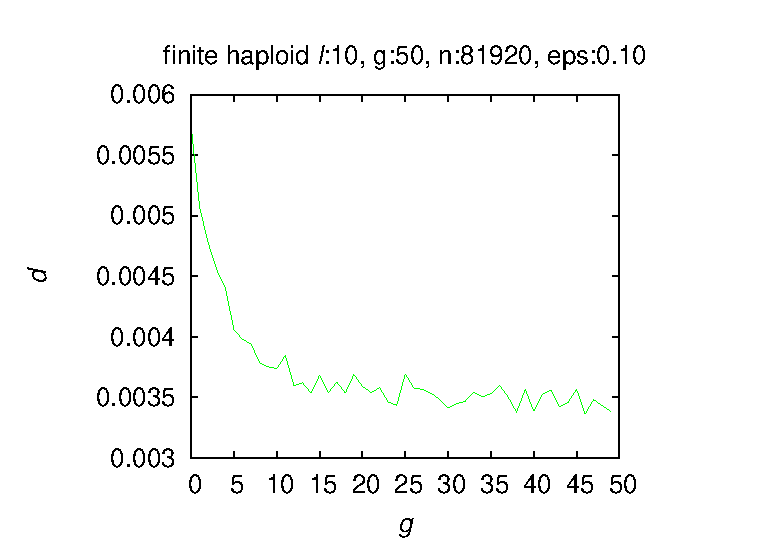
\includegraphics{figures/eps/vio/chi/b10/e0.1/n00081920_fin_hap.eps}}} \hspace{-3em}%
\subfloat{
\resizebox{8cm}{4.5cm}{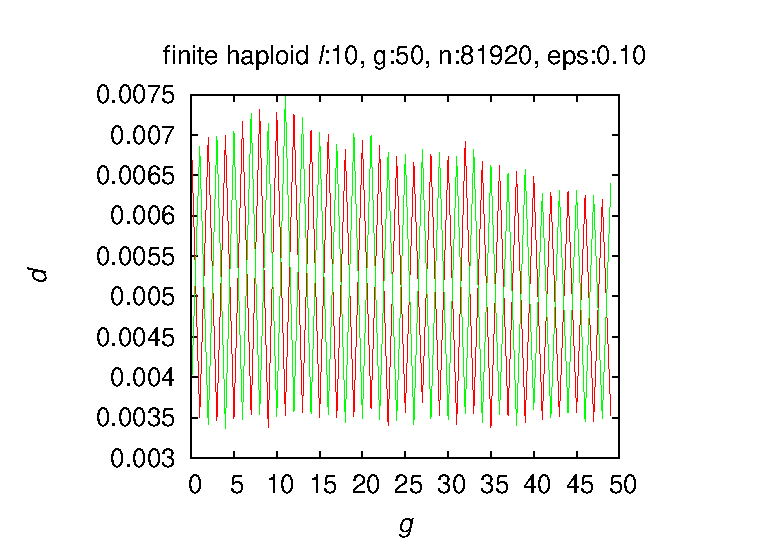
\includegraphics{figures/eps/vio/chi/b10/e0.1/n00081920_fin_hap_wovio.eps}}}\vspace{-1em} \hspace{-3em}%
\end{center}

\begin{center}
\subfloat{
\resizebox{8cm}{4.5cm}{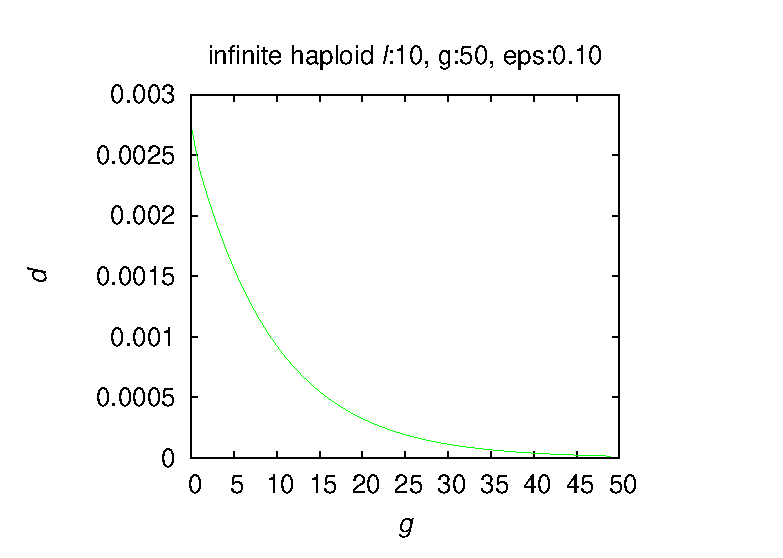
\includegraphics{figures/eps/vio/chi/b10/e0.1/inf_hap.eps}}}\hspace{-3em}%
\subfloat{
\resizebox{8cm}{4.5cm}{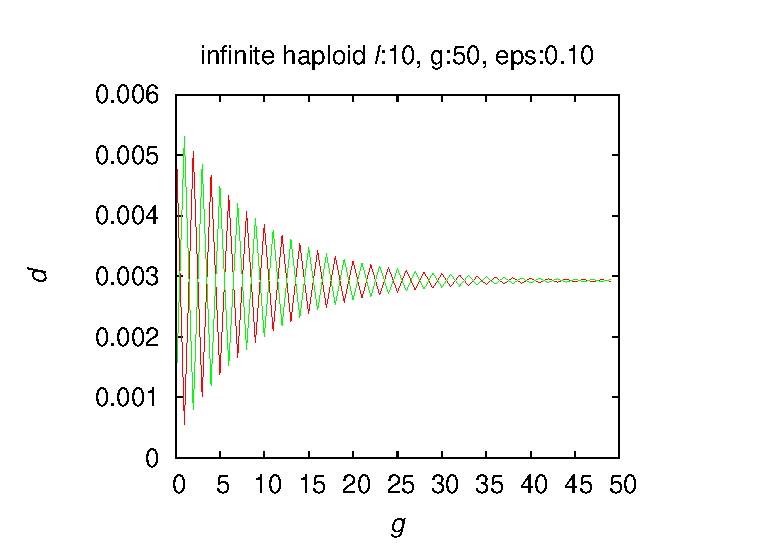
\includegraphics{figures/eps/vio/chi/b10/e0.1/inf_hap_wovio.eps}}}\vspace{-0.5em} \hspace{-3em}%

\caption[\textbf{Infinite and finite haploid population behavior for $\bm{\chi}$ violation, genome length $\ell = 10$ and $\bm{\epsilon} = 0.1$}]{\textbf{Infinite and finite haploid population behavior for $\bm{\chi}$ violation, genome length $\ell = 10$ and $\bm{\epsilon} = 0.1$:} 
  In left column, $d'$ is distance of finite or infinite population to limit $\bm{z}^\ast$ for $g$ generations. In right column, $d$ is distance of finite or infinite population to limits $\bm{p}^\ast$ and $\bm{q}^\ast$. Green line is distance to $\bm{p*}$ and red line is distance to $\bm{q*}$.}
\label{oscillation_10h_vio_chi_0.1}
\end{center}
\end{figure}


% l = 12
\begin{figure}[h]
\begin{center}
\subfloat{
\resizebox{8cm}{4.5cm}{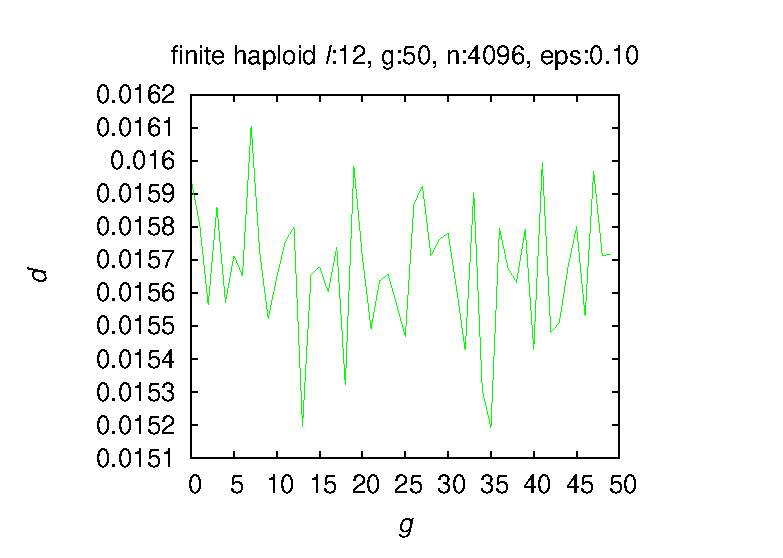
\includegraphics{figures/eps/vio/chi/b12/e0.1/n00004096_fin_hap.eps}}} \hspace{-3em}%
\subfloat{
\resizebox{8cm}{4.5cm}{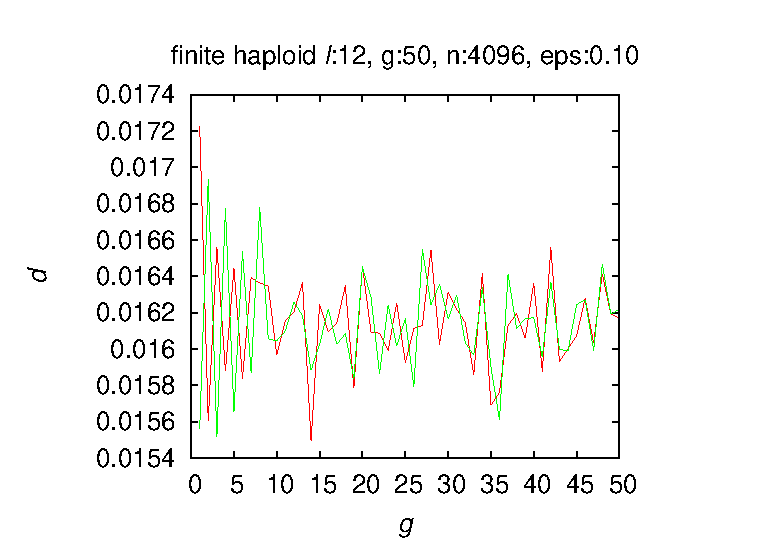
\includegraphics{figures/eps/vio/chi/b12/e0.1/n00004096_fin_hap_wovio.eps}}}\vspace{-1em} \hspace{-3em}%
\end{center}
\begin{center}
\subfloat{
\resizebox{8cm}{4.5cm}{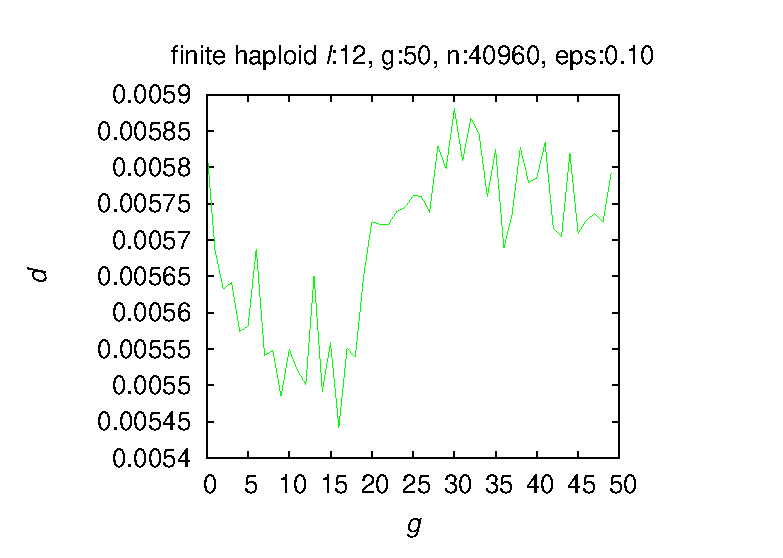
\includegraphics{figures/eps/vio/chi/b12/e0.1/n00040960_fin_hap.eps}}} \hspace{-3em}%
\subfloat{
\resizebox{8cm}{4.5cm}{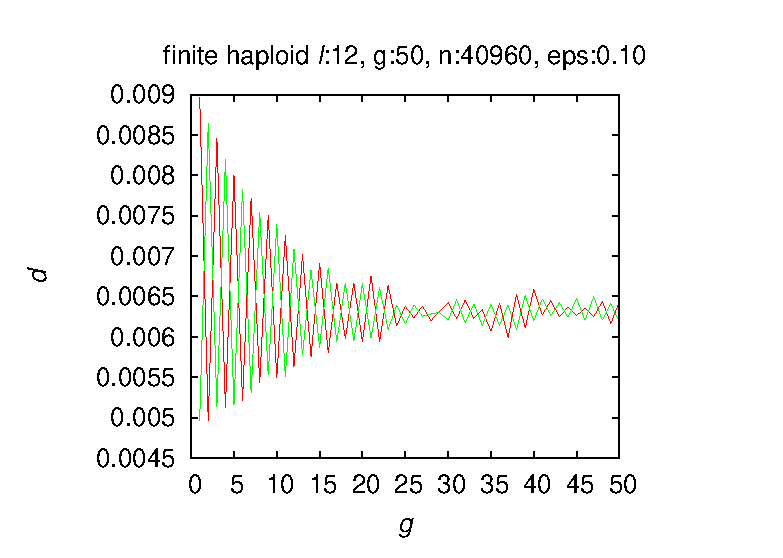
\includegraphics{figures/eps/vio/chi/b12/e0.1/n00040960_fin_hap_wovio.eps}}}\vspace{-1em} \hspace{-3em}%
\end{center}

\begin{center}
\subfloat{
\resizebox{8cm}{4.5cm}{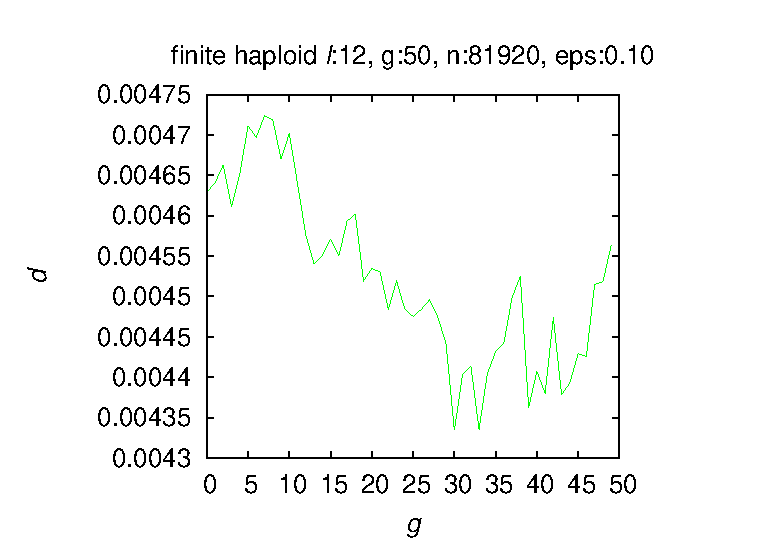
\includegraphics{figures/eps/vio/chi/b12/e0.1/n00081920_fin_hap.eps}}} \hspace{-3em}%
\subfloat{
\resizebox{8cm}{4.5cm}{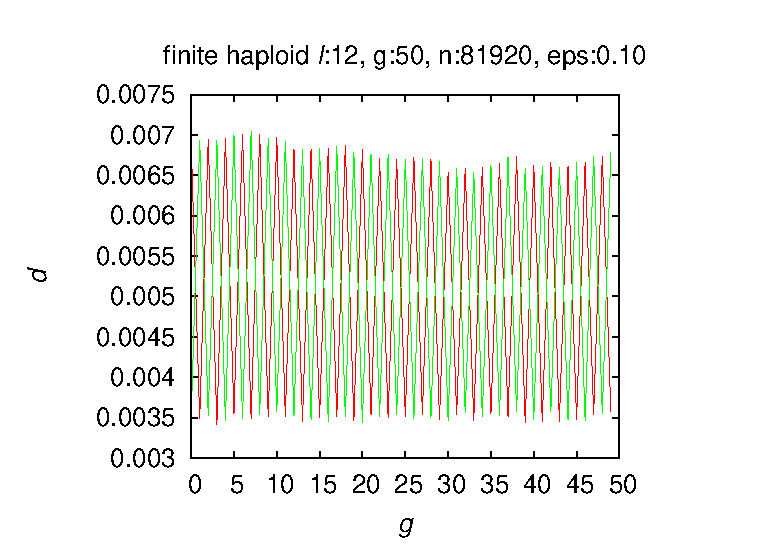
\includegraphics{figures/eps/vio/chi/b12/e0.1/n00081920_fin_hap_wovio.eps}}}\vspace{-1em} \hspace{-3em}%
\end{center}

\begin{center}
\subfloat{
\resizebox{8cm}{4.5cm}{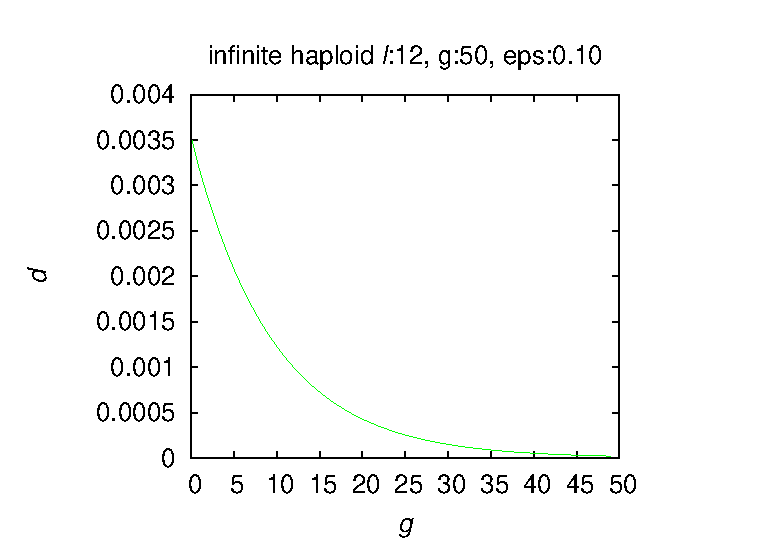
\includegraphics{figures/eps/vio/chi/b12/e0.1/inf_hap.eps}}}\hspace{-3em}%
\subfloat{
\resizebox{8cm}{4.5cm}{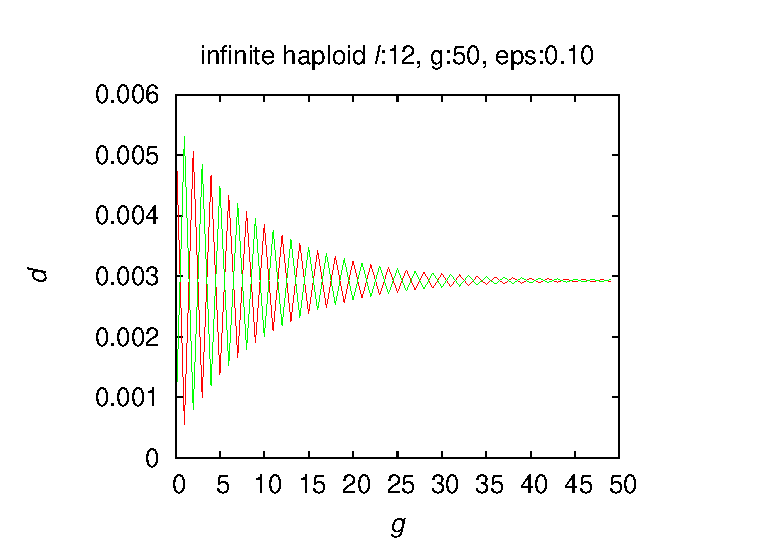
\includegraphics{figures/eps/vio/chi/b12/e0.1/inf_hap_wovio.eps}}}\vspace{-0.5em} \hspace{-3em}%


\caption[\textbf{Infinite and finite haploid population behavior for $\bm{\chi}$ violation, genome length $\ell = 12$ and $\bm{\epsilon} = 0.1$}]{\textbf{Infinite and finite haploid population behavior for $\bm{\chi}$ violation, genome length $\ell = 12$ and $\bm{\epsilon} = 0.1$:} 
  In left column, $d'$ is distance of finite or infinite population to limit $\bm{z}^\ast$ for $g$ generations. In right column, $d$ is distance of finite or infinite population to limits $\bm{p}^\ast$ and $\bm{q}^\ast$. Green line is distance to $\bm{p*}$ and red line is distance to $\bm{q*}$.}
\label{oscillation_12h_vio_chi_0.1}
\end{center}
\end{figure}

% l = 14

\begin{figure}[h]
\begin{center}
\subfloat{
\resizebox{8cm}{4.5cm}{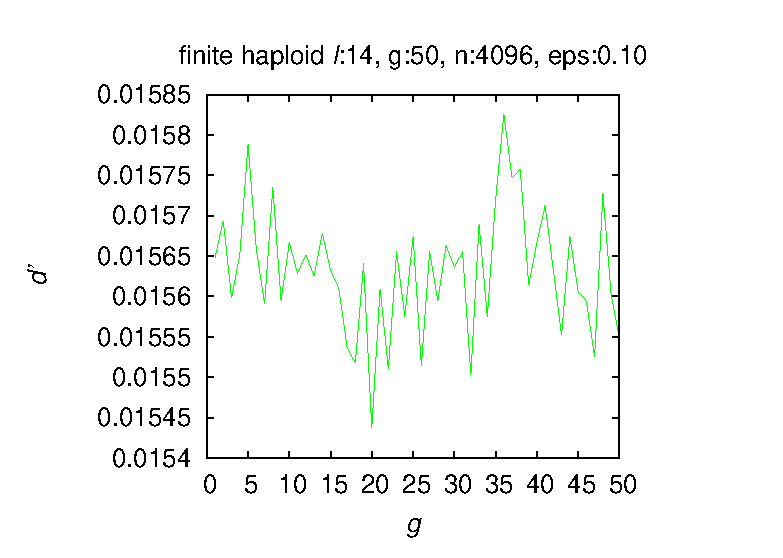
\includegraphics{figures/eps/vio/chi/b14/e0.1/n00004096_fin_hap.eps}}} \hspace{-3em}%
\subfloat{
\resizebox{8cm}{4.5cm}{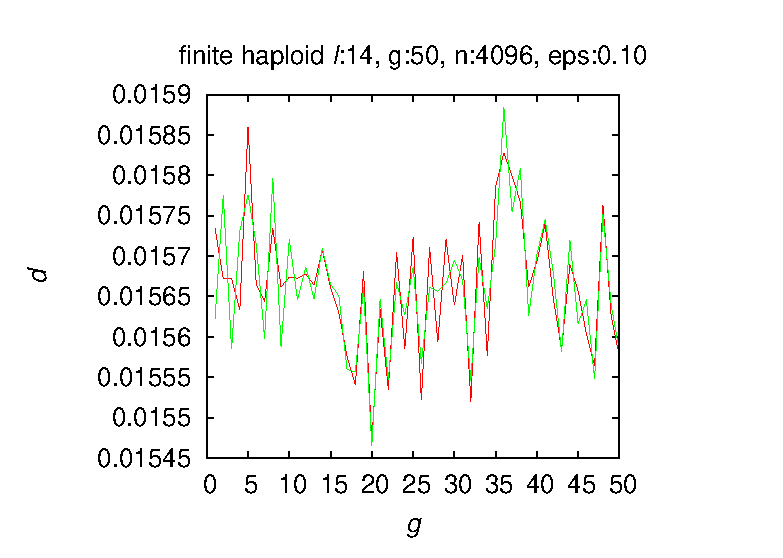
\includegraphics{figures/eps/vio/chi/b14/e0.1/n00004096_fin_hap_wovio.eps}}}\vspace{-1em} \hspace{-3em}%
\end{center}
\begin{center}
\subfloat{
\resizebox{8cm}{4.5cm}{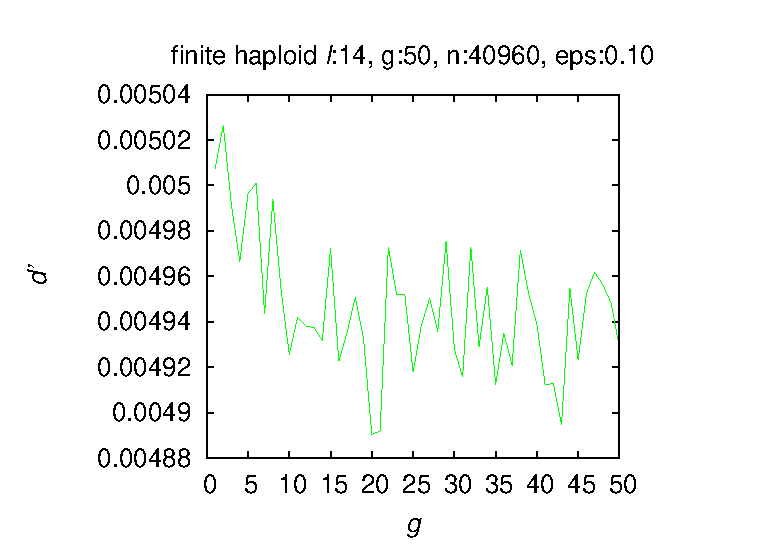
\includegraphics{figures/eps/vio/chi/b14/e0.1/n00040960_fin_hap.eps}}} \hspace{-3em}%
\subfloat{
\resizebox{8cm}{4.5cm}{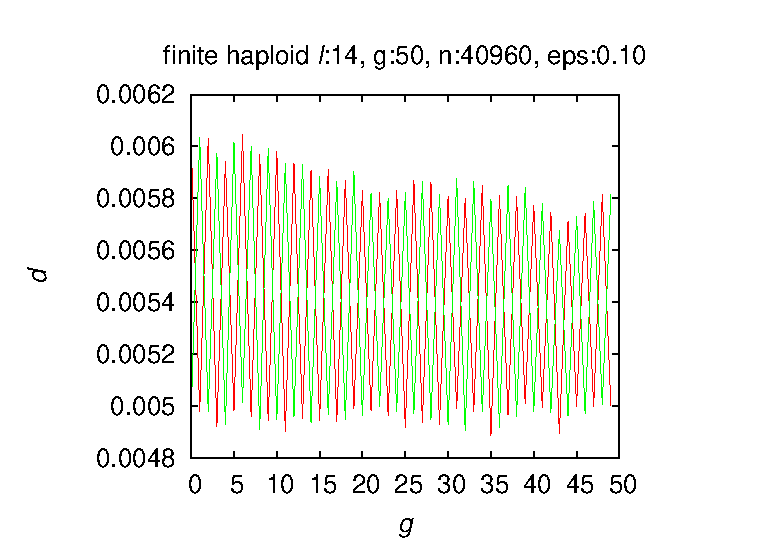
\includegraphics{figures/eps/vio/chi/b14/e0.1/n00040960_fin_hap_wovio.eps}}}\vspace{-1em} \hspace{-3em}%
\end{center}

\begin{center}
\subfloat{
\resizebox{8cm}{4.5cm}{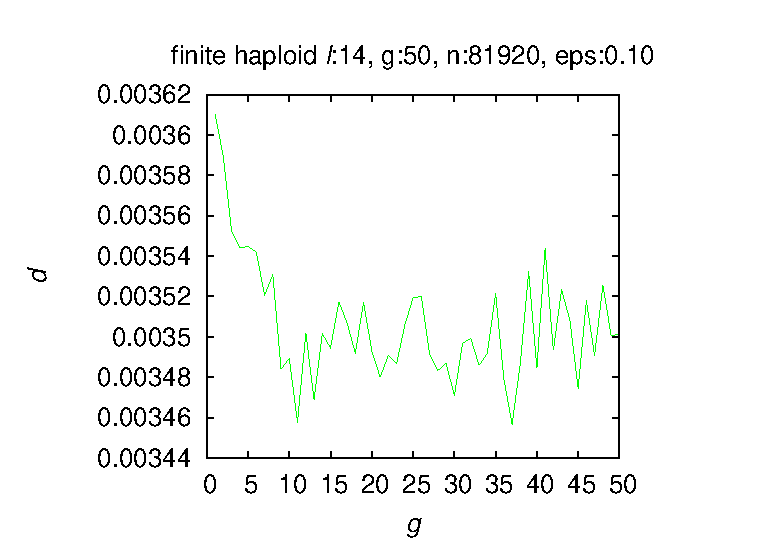
\includegraphics{figures/eps/vio/chi/b14/e0.1/n00081920_fin_hap.eps}}} \hspace{-3em}%
\subfloat{
\resizebox{8cm}{4.5cm}{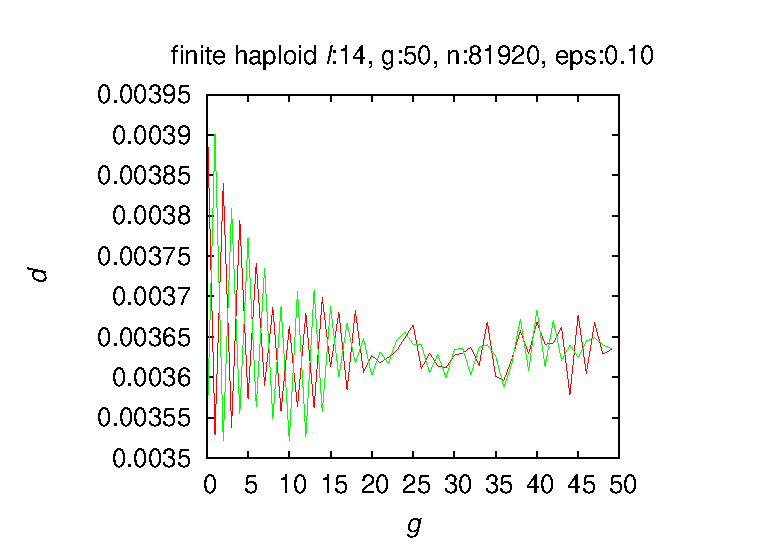
\includegraphics{figures/eps/vio/chi/b14/e0.1/n00081920_fin_hap_wovio.eps}}}\vspace{-1em} \hspace{-3em}%
\end{center}

\begin{center}
\subfloat{
\resizebox{8cm}{4.5cm}{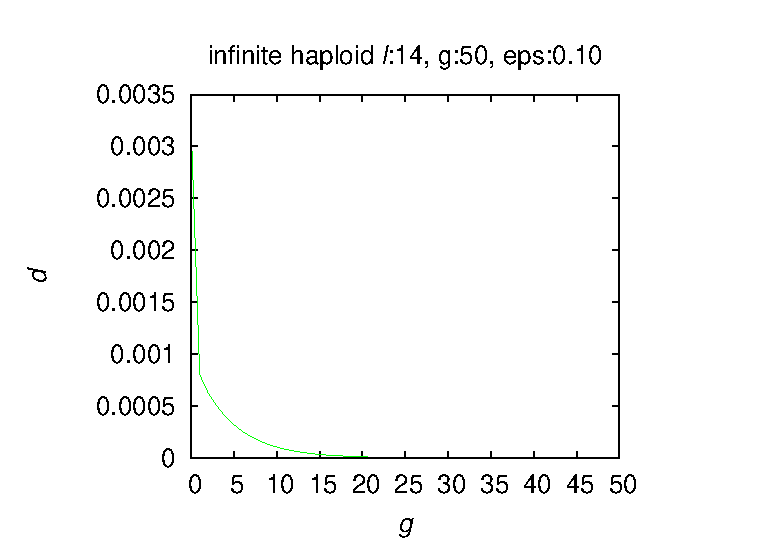
\includegraphics{figures/eps/vio/chi/b14/e0.1/inf_hap.eps}}}\hspace{-3em}%
\subfloat{
\resizebox{8cm}{4.5cm}{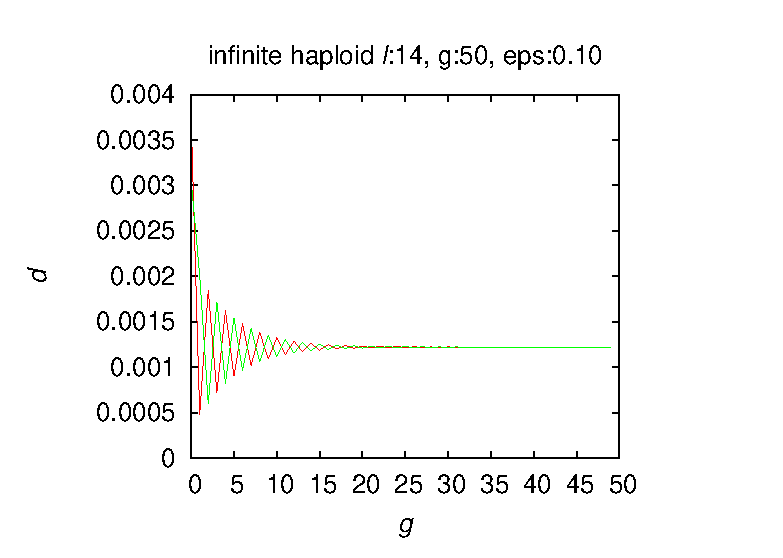
\includegraphics{figures/eps/vio/chi/b14/e0.1/inf_hap_wovio.eps}}}\vspace{-0.5em} \hspace{-3em}%

\caption[\textbf{Infinite and finite haploid population behavior for $\bm{\chi}$ violation, $\ell = 14$ and $\bm{\epsilon} = 0.1$}]
{\textbf{Infinite and finite haploid population behavior for $\bm{\chi}$ violation, $\ell = 14$ and $\bm{\epsilon} = 0.1$:} 
  In left column, $d'$ is distance of finite or infinite population to limit $\bm{z}^\ast$ for $g$ generations. 
  In right column, $d$ is distance of finite or infinite population to limits $\bm{p}^\ast$ and $\bm{q}^\ast$. Green line is distance to $\bm{p*}$ and red line is distance to $\bm{q*}$.}
\label{oscillation_14h_vio_chi_0.1}
\end{center}
\end{figure}

% \clearpage
The right column in figures \ref{oscillation_8h_vio_chi_0.1} through \ref{oscillation_14h_vio_chi_0.1} 
shows distance of finite and infinite haploid populations to non-violation limits $\bm{p^\ast}$ and $\bm{q^\ast}$ with $\bm{\epsilon} \;=\; 0.1$. 
Those graphs indicate oscillating behavior which decreases with time. 
For $\bm{\epsilon} \;=\; 0.1$, infinite population oscillation dies out quickly, 
but oscillation in finite population does not. Rate of damping of ripples with $\bm{\epsilon} \;=\; 0.1$ is  
larger than with $\bm{\epsilon} \;=\; 0.01$. 
The new mask with probability $\bm{\epsilon} \;=\; 0.1$ has  
probability of being used during crossover too small to disrupt oscillation in finite populations. 

The left column of figures \ref{oscillation_8h_vio_chi_0.1} through \ref{oscillation_14h_vio_chi_0.1} 
shows distance of finite and infinite haploid populations to limit $\bm{z^\ast}$ 
when $\bm{\epsilon} \;=\; 0.1$. 
The distance decreases as population size increases, 
and finite population behavior is similar to infinite population as population size grows. 
Average distance data for haploid population in case of violation in $\bm{\chi}$ distribution 
with $\bm{\epsilon} \;=\; 0.1$ are tabulated in table \ref{distanceChiHapEps0.1}.

\clearpage
\begin{table}[h]
\caption[\textbf{Distance measured for violation in $\bm{\chi}$ with $\bm{\epsilon} \;=\; 0.1$  for haploids}]{\textbf{Distance measured for violation in $\bm{\chi}$ with $\bm{\epsilon} \;=\; 0.1$  for haploids:} $\ell$ is genome length, 
average distance between finite and infinite population is tabulated in the last three columns, and last row is expected single step distance.}
\centering
\begin{tabularx}{0.75\textwidth}{ c *{3}{X}}
\toprule
$\ell$ & $N = 4096$ & $N = 40960$ & $N = 81920$  \\
\midrule
8 & 0.0163	& 0.0061 	& 0.0051 \\
10 & 0.0157	&  0.0051	& 0.0037 \\	
12 & 0.0157	&  0.0051	& 0.0037 \\	
14 & 0.0156	&  0.0049	& 0.0035 \\
\midrule
$1/\sqrt{N}$ & 0.0156 & 0.0049 & 0.0035 \\
\bottomrule
\end{tabularx}
\label{distanceChiHapEps0.1}
\end{table} 
Table \ref{distanceChiHapEps0.1} shows that the average distance 
between finite and infinite populations decreases with increasing string length 
approaching the expected single step distance $1/\sqrt{N}$. 
